\documentclass[10pt,twocolumn,letterpaper]{article}

\usepackage{cvpr}
\usepackage{times}
\usepackage{epsfig}
\usepackage{graphicx}
\usepackage{amsmath}
\usepackage{amssymb}

\usepackage{rotating}
\usepackage{graphicx}

% Include other packages here, before hyperref.

% If you comment hyperref and then uncomment it, you should delete
% egpaper.aux before re-running latex.  (Or just hit 'q' on the first latex
% run, let it finish, and you should be clear).
\usepackage[pagebackref=true,breaklinks=true,letterpaper=true,colorlinks,bookmarks=false]{hyperref}

\cvprfinalcopy % *** Uncomment this line for the final submission

\def\cvprPaperID{****} % *** Enter the CVPR Paper ID here
\def\httilde{\mbox{\tt\raisebox{-.5ex}{\symbol{126}}}}

% Pages are numbered in submission mode, and unnumbered in camera-ready
\ifcvprfinal\pagestyle{empty}\fi
\begin{document}

%%%%%%%%% TITLE
\title{Project Report: CS 7643 Hateful Memes Detection}

\author{Yi Gu\\
ygu308\\
{\tt\small ygu308@gatech.edu}
% For a paper whose authors are all at the same institution,
% omit the following lines up until the closing ``}''.
% Additional authors and addresses can be added with ``\and'',
% just like the second author.
% To save space, use either the email address or home page, not both
\and
Wenlei Li\\
wli491\\
{\tt\small wli491@gatech.edu}
\and
Ning Qiao\\
nqiao6\\
{\tt\small nqiao6@gatech.edu}
\and
Stephen Wang\\
swang774\\
{\tt\small stephen.wang@gatech.edu}
}

\maketitle
%\thispagestyle{empty}

%%%%%%%%% ABSTRACT
\begin{abstract}
   Starting from pre-trained baseline models, our work focused on exploring a variety of ways to improve model performances in detecting hateful speech in multimodal memes. We utilized four primary approaches: 1) Utilizing external datasets to increase the training size for the model. 2) Fine-tuning pre-trained models on the specific Multimodal hateful Memes Detection Tasks. 3) Replacing the underlying encoders of baseline models from Bert to Roberta embedding. 4) Using ensemble models to improve final prediction performances.
   
   The final ensembled multimodal models have all achieved an ROC-AUC above 74\% (Highest: 75.33\%) for the test set, which  is a 3-4\%  improvement over the best model baseline (71.41\%). We also provide insights and statistics to better analyze pros and cons of different approaches in hateful meme detection.
\end{abstract}

%%%%%%%%% BODY TEXT
\section{Introduction/Background/Motivation}

Social media is becoming a major part of our everyday life. It makes communication easier and spreads information faster than ever before. It can also be used for hate speech - used to “attack a person or a group on the basis of who they are, in other words, based on their religion, ethnicity, nationality, race, color, descent, gender or other identity factor”~\cite{Authors1}.

Multimodal hateful memes, which often combine text and images together have become a new way for people to spread hateful speech. Although there have been unimodal-based AI models applied in the field of hate speech detection, models that rely on just text or just images to determine whether or not a meme is hateful are insufficient, due to the fact that the text or image of the meme may seem neutral if looked at individually but becomes hate speech when viewed together with the others. Currently, The state-of-the-art methods perform poorly compared to humans (64.73\% vs. 84.7\% accuracy).~\cite{Authors1} Therefore, multimodal hate speech detection remains a difficult technical challenge.

This work focuses on applying a variety of multimodal algorithms and their combinations in the aim of improving deep learning  model performance in multimodal hateful meme detection, which can not only help advance multimodal deep learning systems but can also possibly be utilized by social media platforms as a practical approach in automatically detecting and removing hateful speech. This helps to build a more peaceful online environment, as such hateful speech often serves as a catalyst in instigating hateful crime and social polarization.

The \href{https://www.drivendata.org/competitions/64/hateful-memes/data/}{Dataset} used is "The Hateful Memes Challenge Set" provided by Facebook Artificial Intelligence (AI). The Dataset has been specifically reconstructed, filtered, reproduced, rated and annotated for the challenge of multimodal hateful meme detection.~\cite{Authors2}

The Dataset also includes specially created "Benign Confounders" examples, which are "a minimum replacement image or replacement text that flips the label for a given multimodal meme from hateful to non-hateful."~\cite{Authors2}. This particular feature has made the dataset more challenging and would force the model to make predictions based on multimodality in order to have better performance.

The full Dataset comprises of 10K unique named data points, which covers five different types of memes: multimodal hate, unimodal hate, benign image and benign text confounders, and finally random not-hateful examples. 
~\cite{Authors2}

The dataset has been split into training(85\%), dev(5\%) and test(10\%) sets."The dev and test set are fully balanced, and are comprised of memes using the following percentages: 40\% multimodal hate, 10\% unimodal hate, 20\% benign text confounder, 20\% benign image confounder, 10\% random non-hateful.In the competition phase 2, the dev and test set has been updated to the dev\_unseen and test\_unseen of size 540 and 2000 respectively.

During our investigation, we used the training set(8500) and dev\_unseen(540) set for model fine-tuning and cross-validation and the test\_seen\footnote{We are using the smaller test\_seen set of size 1000 due to the fact that the dataset does not provide ground truth labels for test sets and the final test performance can only be evaluated by submitting the result to the competition. In our work, only phase 1 of the competition which uses test\_seen set to evaluate the final performance is available.} set for testing the final model performance evaluation.

In addition to the Hateful Memes data, we found a hateful memes dataset that contains 328 labeled memes by one of the top competitors - Team HateDetectron in the Hateful Memes Phase 2 competition. We have added these 328 memes to the Visual BERT (with and without CC transfer learning) models’ training sets. See \textbf{Section 2.1} for more details.

%-------------------------------------------------------------------------
%------------------------------------------------------------------------
\section{Approach}
Starting from pre-trained baseline models, we have followed four major approaches below to explore different methods in improving multimodal performances in Hateful Memes Detection task.

Given that the structure of the hateful memes are multimodal in nature (text and images), all of our models employed are multimodal models which performs joint representation for vision and language. For instance, VisualBERT model fuses both the Transformer based BERT embedding and a visual embedding. ~\cite{Authors5} These structures are necessary for the models to successfully consider both text and image content when determining whether a meme is hateful. 

Throughout our work, we have utilized the \href{https://github.com/facebookresearch/mmf}{MMF repository} provided by Facebook and followed the sample procedure available \href{https://colab.research.google.com/github/facebookresearch/mmf/blob/notebooks/notebooks/mmf_hm_example.ipynb#scrollTo=ulosPHAE-eto}{here} in employing pre-trained models and checkpoints, performing model fine-tuning and training as well as replacing encoders.

\subsection{Dataset Expansion}
One of the approaches we applied was to add more data to the training set. If the quality of data is good, larger datasets usually result in better models. Using a small dataset with a complex model may result in overfitting and higher estimation error. After a bit of searching, we found one of the top competitors - Team HateDetectron in the Hateful Memes Phase 2 competition labeled 328 memes for the Phase 2 competition. The original dataset - the “Memotion Dataset” - contains 14 thousand memes from the SemEval “Memotion Analysis” challenge in 2020. The Memotion Dataset is open-sourced and can be downloaded \href{https://www.kaggle.com/williamscott701/memotion-dataset-7k}{here}. The Memotion Dataset is labeled with sentiments as motivational, offensive, sarcastic, and humorous. Team HateDetectron discovered that the dataset is incorrectly labeled and cherry-picked and truth (labeled) 328 the memes that would be suitable for the Hateful Memes challenge.~\cite{Authors3}. The repository for the 328 labeled memes and ingest code can be found \href{https://github.com/rizavelioglu/hateful_memes-hate_detectron}{here}. See example in \textbf{Figure 1}. Out of 328 memes, 107 memes were labeled as positive and 221 memes labeled as negative. The Open-sourced dataset memes have similar balance as the Hateful Memes Challenge Set. The combination of the Hateful Memes Challenge Set training data and the additional Memotion Dataset labeled dataset made up 8828 memes in the training set. The training/validation/test split with the additional data is 85.5\%,9.68\% and 4.8\%.

\begin{figure}[ht!]
\centering
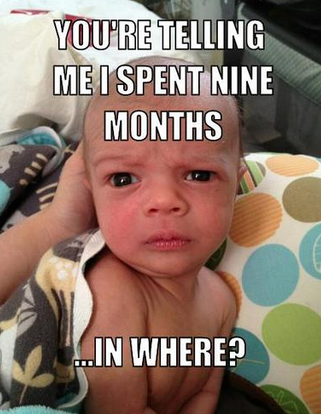
\includegraphics[scale=0.5]{images/new_meme.png}
\caption{Example additional meme}
\end{figure}

We added the dataset expansion on the Visual BERT (with and without transfer learning) models’ training sets. We then applied fine-tuning to the Visual BERT results and saw an improvement after applying COCO or CC transfer learning. See \textbf{Section 3.1} for a subset of fine-tuned results.

\subsection{Fine-tuning on Pre-trained Baseline Model}
In order to avoid reinventing the wheel, we first tried to improve the performance of the Hateful Memes detection by continuing to fine-tune multimodally pretrained versions in the ViL BERT CC(trained on Conceptual Captions) and Visual BERT COCO (trained on COCO). One of the reasons is that both ViL BERT CC and Visual BERT COCO performed better than other multimodal/unimodal models according to the baseline model performance result~\cite{Authors2}. In addition, these two models have been pretrained on lager multimodal dataset(CC, COCO) and we could transferred their learned knowledge through fine-tuning to solve the similar Hateful Memes detection issue. Due to the computing resource limitation(1 GPU, 16/25G RAM), we limited batch size under 48 to fine-tune these models. According to the experimental results (see \textbf{Section 3.1}), we have indeed obtained better results on AUROC and Accuracy than their baseline models.

We also tuned the parameters of Unimodal/Multimodal (Unimodal Pretraining) baseline models (Image-grid, Text BERT, Visual BERT, ViL BERT) and retrained them on the default Hateful Memes dataset. The retrained models did not outperform based on our experiment results, but they did help us to better understand the data set, different classifiers/models performance, and find ways to design new models and/or assemble the current models. 

We performed hyperparameter tuning over the batch size, max updates, learning rate, number of classifier layers(for unimodal models only) and scheduler related parameters. See Table 1 for more details. 

\subsection{Replacing BERT Encoder with RoBERTa}
Introduced by Facebook, RoBERTa is a refined version of BERT model which incorporated refinement techniques such as pre-training on larger dataset, removing the Next Sentence Prediction objective and introducing dynamic masking etc.~\cite{Authors4}  

Starting upon the baseline Visual BERT model pre-trained on COCO, we have utilized the RobERTa tokenizer originally posted from this \href{https://github.com/pytorch/fairseq/tree/master/examples/roberta} {repository} to replace the default BERT tokenizer, and preformed fine-tuning experiments specifically on completing the Hateful Memes task, which we believe would be a possible way in improving model performances by using improving embedding tokenizer.

Compared to BERT encoder, the RoBERTa tokenizer have used a larger sequence size and employed dynamic masking. All this has introduced a significantly larger amount of parameters to tune with corresponding more powerful computational resource demanded. During the hyper-parameter tuning we encountered an issue - the 12Gb memory limit of Colab is insufficient for the model to train. Upgrading to Colab pro with 25Gb of RAM plus and 16Gb GPU can only handle a largest batch size around 54-56. Tuning a larger batch size will require to switch to a 35Gb RAM.

Therefore, for this approach, the computational resource is an important factor to consider. The fine-tuning results and analysis for RoBERTa model can be found in \textbf{Section 3.2}.

\subsection{Ensembling}
After the above efforts, we decided to leverage Ensemble learning methods to produce joint predictions from our best performing models, which is one of the major techniques used in machine learning, combing the benefits of different models and smoothing the prediction curves.

To accommodate with the submission format of the competition, we manually coded our ensemble functions to evaluate and generate the required ensembled predictions for both dev and test sets. 

There are two types of ensembling methods employed:  Soft Ensemble and Hard Ensemble, where the soft methods makes predictions based on the average probability of each individual model, while the hard mode makes predictions based on average hard binary labels of each individual models. 

We have performed the analysis on 34 total different combinations of our individually trained models. And have chosen the best among them to make predictions on the tests set. Our final ensemble model performances and analysis were summarized in \textbf{Section 3.3}

\section{Experiments and Results}
This section summarizes the experiments and results from different approaches and final performance for ensemble models.

During training, the optimizer is based on the Adam algorithm, and the loss is measured by cross-entropy loss. The model parameters/weightings learned are generally for the transformer layers, embedding layers as well as final classifier layers. Other specific important hyper-parameters being tuned are illustrated in each individual section below.

The final results were measured based on AUROC and prediction Accuracy which aligns with the competition requirements found \href{https://www.drivendata.org/competitions/64/hateful-memes/submissions/}{here}.

\subsection{Fine-tuning on Pre-trained Baseline Model}

The results are shown in \textbf{Table 1}. 

Among the parameters used in our experiment (see Table 1) with the default Hateful Memes dataset, for the unimodal models, the performance(Accuracy and/or AUROC) of Text BERT(on average $>$0.6) is slightly better than that of Image-Grid(on average $<$0.6), which shows the performance of text-only classifier under unimodal slightly better than visual-only classifier; For the multimodal(unimodal pretraining) models, the best performance of Visual BERT(AUROC: 0.7141) is better than the best performance of ViL BERT(AUROC: 0.6881), which shows that the performance of these two vision-and-text combined classifiers is slightly different; For the multimodal(multimodal pretraining) models,  the best performance of Visual BERT COCO(AUROC: 0.7428) is better than the best performance of ViL BERT CC(AUROC: 0.7064); Among all the above models, the multimodal model Visual BERT COCO works best for AUROC. It’s far better than the unimodal models in performance. It may be because of the advantage of the transferring learning, the unbalanced Hateful Memes training data and/or we haven’t tuned parameters enough in our experiments. The performance of these baseline models can probably be improved further. The best Visual BERT COCO was restrained on the default Hateful Memes dataset with batch size 32 and maximum update 15000, we got AUROC 0.7428 and Accuracy 0.7 on the validation dataset, and AUROC 0.7330(better than the baseline model's 0.7141) and Accuracy 0.652 on the test dataset (submission result on DrivenData - Hateful Memes: Phase 1).

As previously stated in 2.1, we incorporated 328 labeled memes from the Memotion Dataset. We add the additional data to the training set and focus our fine-tuning on the Visual BERT COCO model because it performed the best out of all the models we fine-tuned earlier. Besides Visual BERT model with COCO pre-trained, we also tested the Visual BERT model with Conceptual Caption (CC) pre-trained set. We noticed a significant improvement in the performance, mainly on the AUROC metric.

The best-fine-tuned result with the additional training data is 0.7500 AUROC with 0.7204 Accuracy on the validation dataset and 0.7395 AUROC with 0.644 Accuracy on the test dataset (submission result on DrivenData - Hateful Memes: Phase 1). The model has higher validation AUROC and Accuracy but only slightly better in test AUROC and marginally worse in test Accuracy compared to the default set model shows possible overfitting in the model.

During the fine-tuning, we also found that the smaller learning rate (model converges slower) performed slightly better than the larger learning rate(e.g. lr 1e-4 vs le-5 for ViL BERT) and the larger batch size(model converge faster) performed slightly better than smaller batch size(e.g. Batch size 32 vs 16 for Visual BERT COCO). Another observation we had is that pre-trained models reach the best iterations (local minima) much faster. 

We can see that fine-tuning especially the multimodal (multimodal pretraining) baseline models do have high possibility to improve the performance of Hateful Memes detection. This encourage us to think further. Could we make a signal model better by expanding to even more training data (328 more memes is only 0.5\% of total data)? Can we modify the baseline models(e.g. encoder) to achieve better performance? Can we ensemble these relatively weaker learners to build stronger learners? Therefore, we decided to archive our goal to improve the performance a little bit via a fine-tuning method on each single model and then use them as a part of the ensemble models to get the best result in our project.


\begin{table*}[h]
\begin{center}
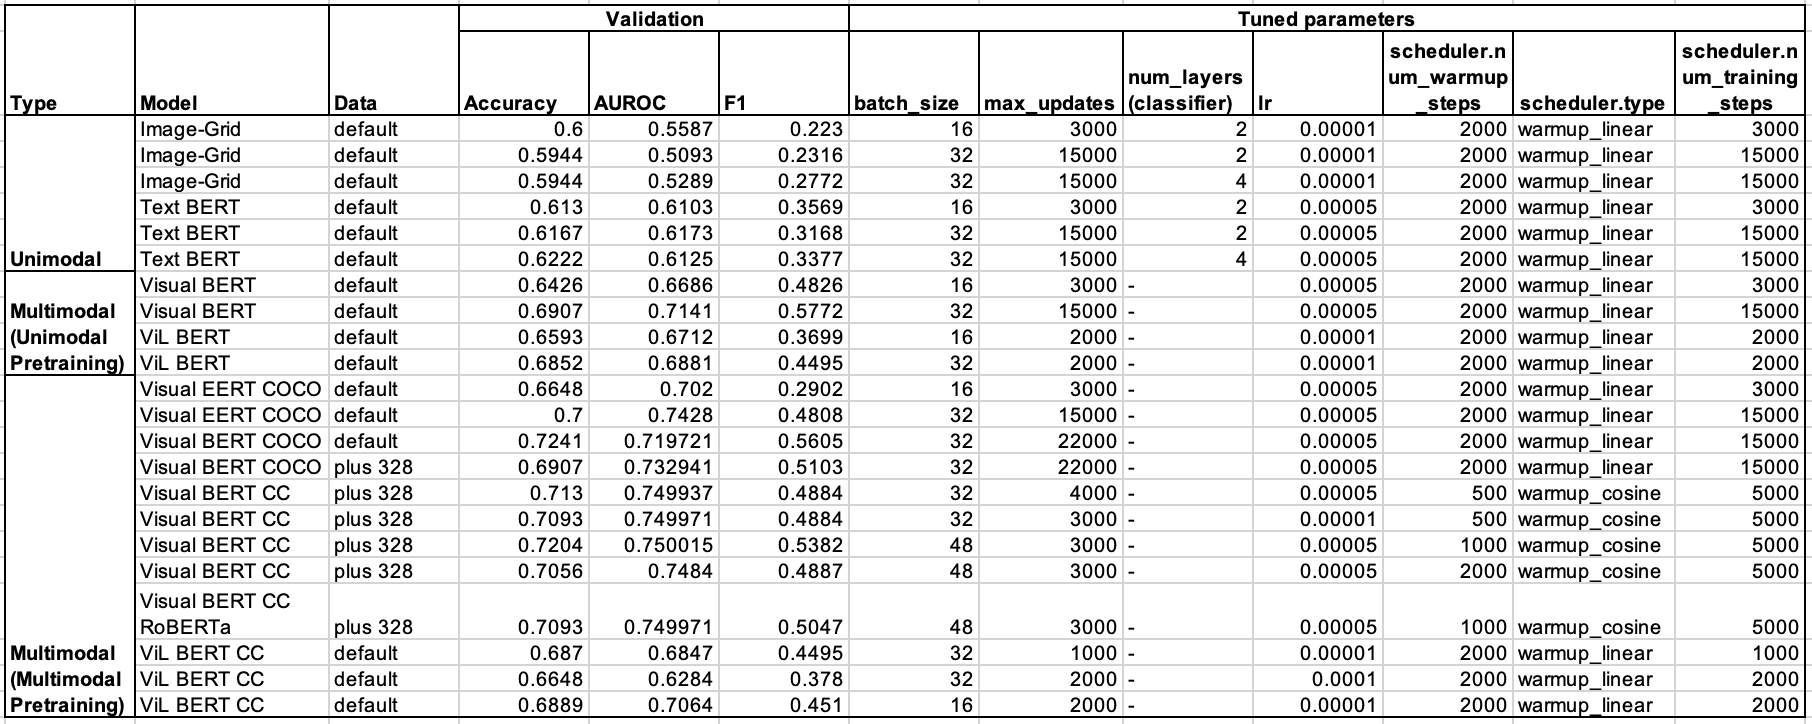
\includegraphics[scale=0.58]{images/fine-tuned.png}
\caption{A Subset of Fine-tuned Results}
\end{center}
\end{table*}

\subsection{Replacing BERT Encoder with RoBERTa}
As shown in \textbf{Table 2}, the important hyper-parameters that has been tuned are Batch Size, Learning Rate, Mask Probability, Max Updates and Max Sequence Length. 

It is observed that with a relatively larger batch size, the model trains and convergences in a relatively more stable and smoother manner, and achieves a better performance for validation set. However, due to the computational limits for Colab Pro GPUs, the largest batch size can be handled is around 56, as mentioned previously. We thus choose a batch size of 56 to best leverage between training time and model performance. 

Also, we have found that increasing the learning rate slightly from 5e-5 to 1e-4 can help the learning process to achieve more stable higher AUROC and accuracy. 

By utilizing the pre-trained model weights from COCO, the training of RoBERTa model converges relatively fast, after around 2000 updates, the validation CE loss tend to reach the minimum and keep training the model does not bring further improvement in terms of accuracy and there are over-fitting scenarios observed where training loss decreases while validation loss actually increase. Therefore, 3000 max updates is sufficient in training and the best performing model are located at around 1850 updates for the best hyper-parameter combinations. 

Applying the mask probability could bring some improvements to model performance as well. This could possibly be contributed to the benefits of the dynamic masking mechanisms of RoBERTa model. Also, decreasing the max sequence length does not seem to help with model performances. This could be due to two possible reasons: 1. A sequence length of 56 is not sufficient to cover enough text information and causes some useful information to be discarded. 2. The smaller sequence length cannot fully utilize the benefits introduced by RoBERTa's larger byte-level BPE (Byte-Pair Encoding) subword units.

The best performing model for the hyper-parameter combinations that has been evaluated is highlighted in \textbf{Table 2}. The model achieves a 0.7056 accuracy and 0.722 AUROC of validation set both of which is higher than the baseline model and will be used as a component model for our final ensemble model.


\begin{table*}[h]
\begin{center}
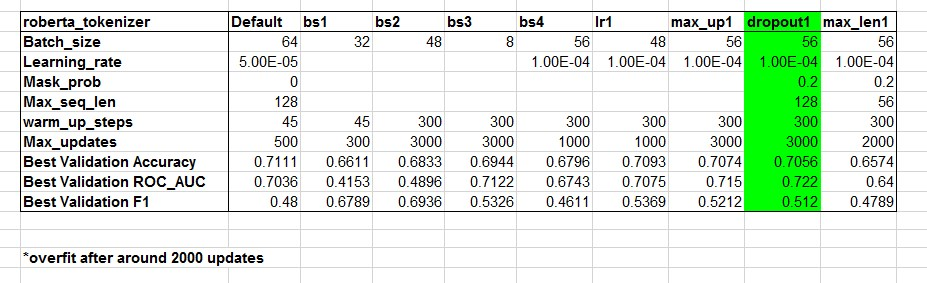
\includegraphics[scale=0.7]{images/roberta.jpg}
\caption{Roberta Model Tuning Results}
\end{center}
\end{table*}


\subsection{Ensembling}
Combining all the pre-trained model baselines and fine-tuned models in Section 3.1 and 3.2, we have tried out 17 groups of models, with both hard and soft ensemble methods, amounting to a total of 34 ensembled models tested and evaluated. The detailed results is shown in \textbf{Table 3}.

We used the Visual BERT pre-trained on COCO model which was then fine-tuned by the expanded dataset as our base model(VBCOCO(aug)), we then added more groups or individual models to form different ensemble combinations and at the same time, we also discarded the individual models or groups that were obviously harming ensembled model performance. For a full list of names of all the component models, please refer to \textbf{Appendix A}.

Then, we followed a hierarchical procedure in distilling ensemble model performance to select the best model combinations. As shown in \textbf{Table 3}, for the ensembled combinations attempts, we use the validation AUROC and Accuracy for our first round of candidate selection: The light green cells signifies tier two candidates, with either measurements of AUROC or Accuracy larger than 70\%, and dark green cells signifies tier one candidates with both AUROC and Accuracy measure larger than 70\%. 

In the second round, we submit the candidate ensemble models in tier one and tier two of total 13 models to the competition for final test set performance evaluation. Based on the final test AUROC and Accuracy, we choose 6 ensemble models highlighted, all of which show an evident advantage over the baseline models in terms of both the AUROC and Accuracy. These test performances are further summarized in \textbf{Table 4}

\begin{table*}[]
\begin{center}
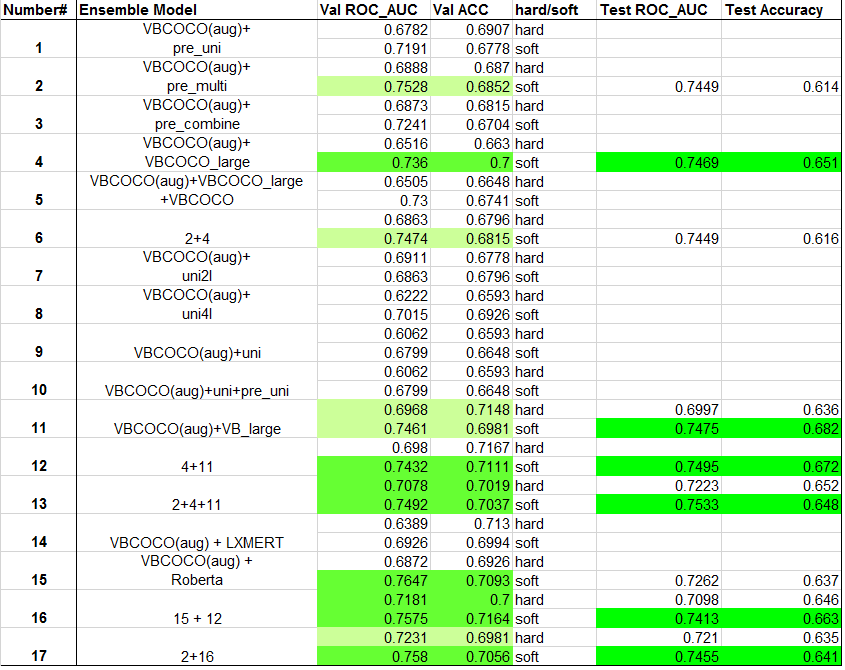
\includegraphics[scale=0.65]{images/Ensemble.png}
\caption{Ensemble Model Results}
\end{center}
\end{table*}

\begin{table*}[]
\begin{center}
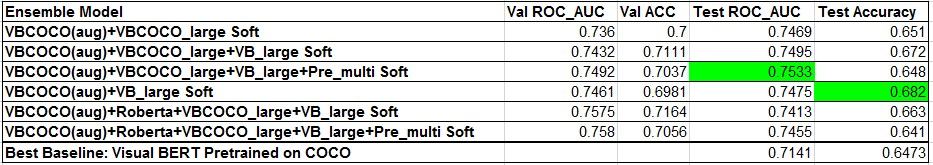
\includegraphics[scale=0.65]{images/Models.jpg}
\caption{Final Selected Model Results}
\end{center}
\end{table*}


\section{Conclusion}
From \textbf{Table 4},which shows the final result of our best ensemble models, we can draw the following observations.

1). The best performing ensemble models are composed of our best individual performing models from different approaches as illustrated in 3.1 and 3.2. This shows the merits of individual approaches of our effort in Data Expansion, Fine Tuning as well as changing the Encoders. 

2). The ensembled model can join the advantages of different component models and bring increase in performance in both test AUROC and Accuracy

3). Adding the pre-trained baseline models to our ensemble predictions can possibly help to generate a more smooth probability prediction curve and thus improve the AUROC measurements. However, this hurts the prediction accuracy for test set a little bit.

4). Adding the baseline models that are pre-trained on unimodal datasets harm the model performances of ensemble models. This further illustrated that the multimodal structures for both the model itself and pre-training teacher tasks are essential for the model to perform well on multimodal hateful memes detection tasks. 

5). The soft ensembling has shown an overall advantage over hard voting methods in terms of both validation and test performance, this is reasonable since the soft voting produce more accurate probability predictions for the final label.

All of our final models outperform the best baseline models by around 3-4\% in AUROC in Test set performance. The highest AUROC achieved is 75.33\% which is 3.92\% higher than the best baseline model; while the highest accuracy achieved is 68.2\%, which is 3.47\% higher than the best baseline model AUROC 71.41\% according to the data available on \href{https://www.drivendata.org/competitions/64/hateful-memes/leaderboard/}{competition website}. Our final model with best AUROC has ranked 69 out 3937 competitors in the Hateful Memes Detection Competition (See Appendix B for screenshot.)


\section{Future Research}
In this project, we proposed four approaches to improve the performance of multimodal hateful memes detection tasks: We utilized more open-source data, applied RoBERTa encoding, fine-tuned pre-trained models, and implemented ensembling with both soft and hard voting. Our final model results show the effectiveness of these approaches as well as their limits, as there is still much  to improve, especially when we compare results to top competitors in the competition and human judgment accuracy. Some possible future experiment directions includes: adding feature extractors that are more specifically related to detecting hateful memes, such as skin tones, religious backgrounds and gender information as well as adding more multimodal models in ensembling: such as UNITER, VILLA-ITM, ERNIE-Vil, OSCAR, DeVLBERT, and etc.


%-------------------------------------------------------------------------
\pagebreak
\onecolumn

{\small
\bibliographystyle{ieee_fullname}
\bibliography{egbib}
}

\appendix
\section*{Appendix}
\section{Ensemble Model Named Lists}
\begin{table}[h]
\begin{center}
\begin{tabular}{|l|l|} 
\hline
Name          & Model                                                                                                                                                                          \\ 
\hline
VBCOCO(aug)   & Fine tuned Visual BERT model pretrained on COCO with additional data~                                                                                                          \\ 
\hline
VBCOCO\_large & Fine tuned Visual BERT model pretrained on COCO with bz 32, max upddate 15000                                                                                                  \\ 
\hline
VB\_large     & Fine tuned Visual BERT~with bz 32, max upddate 15000                                                                                                                           \\ 
\hline
Roberta       & Fine tuned Visual BERT model with RoBERTa Encoder                                                                                                                              \\ 
\hline
pre\_uni      & \begin{tabular}[c]{@{}l@{}}List of Multimodal Baseline Models pretrained on Unimodal Data: \\ConcateBERT, Late Fusion, MMBTGrid, MMBTRegion, ViLBERT, VisualBERT\end{tabular}  \\ 
\hline
pre\_multi    & \begin{tabular}[c]{@{}l@{}}List of Multimodal Baseline Models pretrained on Multimodal Dataset:\\ViLBERT on CC, VisualBERT on COCO\end{tabular}                                \\ 
\hline
pre\_combine  & pre\_multi + pre\_uni                                                                                                                                                          \\ 
\hline
uni2l         & \textcolor[rgb]{0.141,0.161,0.18}{Fine tuned Image-Grid and text BERT model with 2 classifier layers}                                                                          \\ 
\hline
uni4l         & \textcolor[rgb]{0.141,0.161,0.18}{Fine tuned Image-Grid and text BERT model with 4 classifier layers}                                                                          \\
\hline
\end{tabular}
\end{center}
\end{table}


\section{Best Performing Model Rank}
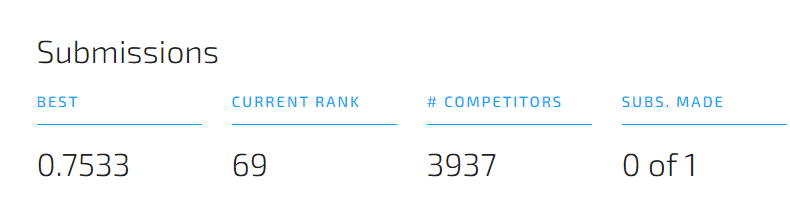
\includegraphics[scale=0.6]{images/ranking.png}

\section{Supplementary Materials}
The code and raw predictions of the models can be found in this \href{https://drive.google.com/drive/folders/1ftH9FxO2Fn0r1WsAlvrzcWtSMJiozbNp?usp=sharing}{folder}

\section{Work Division}
\begin{table}[h]
\begin{center}
\begin{tabular}{|l|c|p{5cm}|}
\hline
Student Name & Contributed Aspects & Sections\\
\hline\hline
Yi Gu & Data Expansion with Visual BERT fine-tuning & Section 2.1, 3,1\\
Wenlei Li & Fine-tuning Image-Grid, Text BERT, Visual BERT and Visual BERT COCO& Section 2.2, 3.1\\
Ning Qiao & Fine-tuning RoBERTa model and model Ensembling & Section 2.3, 2.4, 3.2, 3.3 \\
Stephen Wang & Fine-tuning ViL BERT and ViL BERT with CC & Section 2.2, 3.1 \\
\hline
\end{tabular}
\end{center}
\label{tab:contributions}
\end{table}

%-------------------------------------------------------------------------

\end{document}
